
\documentclass{article}
% Pages are numbered in submission mode, and unnumbered in camera-ready
\usepackage{ctex}
\usepackage{subfigure}
\usepackage{graphicx}
\usepackage{times}
\usepackage{epsfig}
%\usepackage{figure}

\usepackage{amsmath}
\usepackage{amssymb}
\begin{document}
%%%%%%%%% TITLE
\title{ʷ�����ĺ�����}

\author{��������Խ~~~ѧ�ţ�1600012704}

\maketitle
\section{Section one}

    \begin{figure}
		\begin{center}
		\subfigure{
		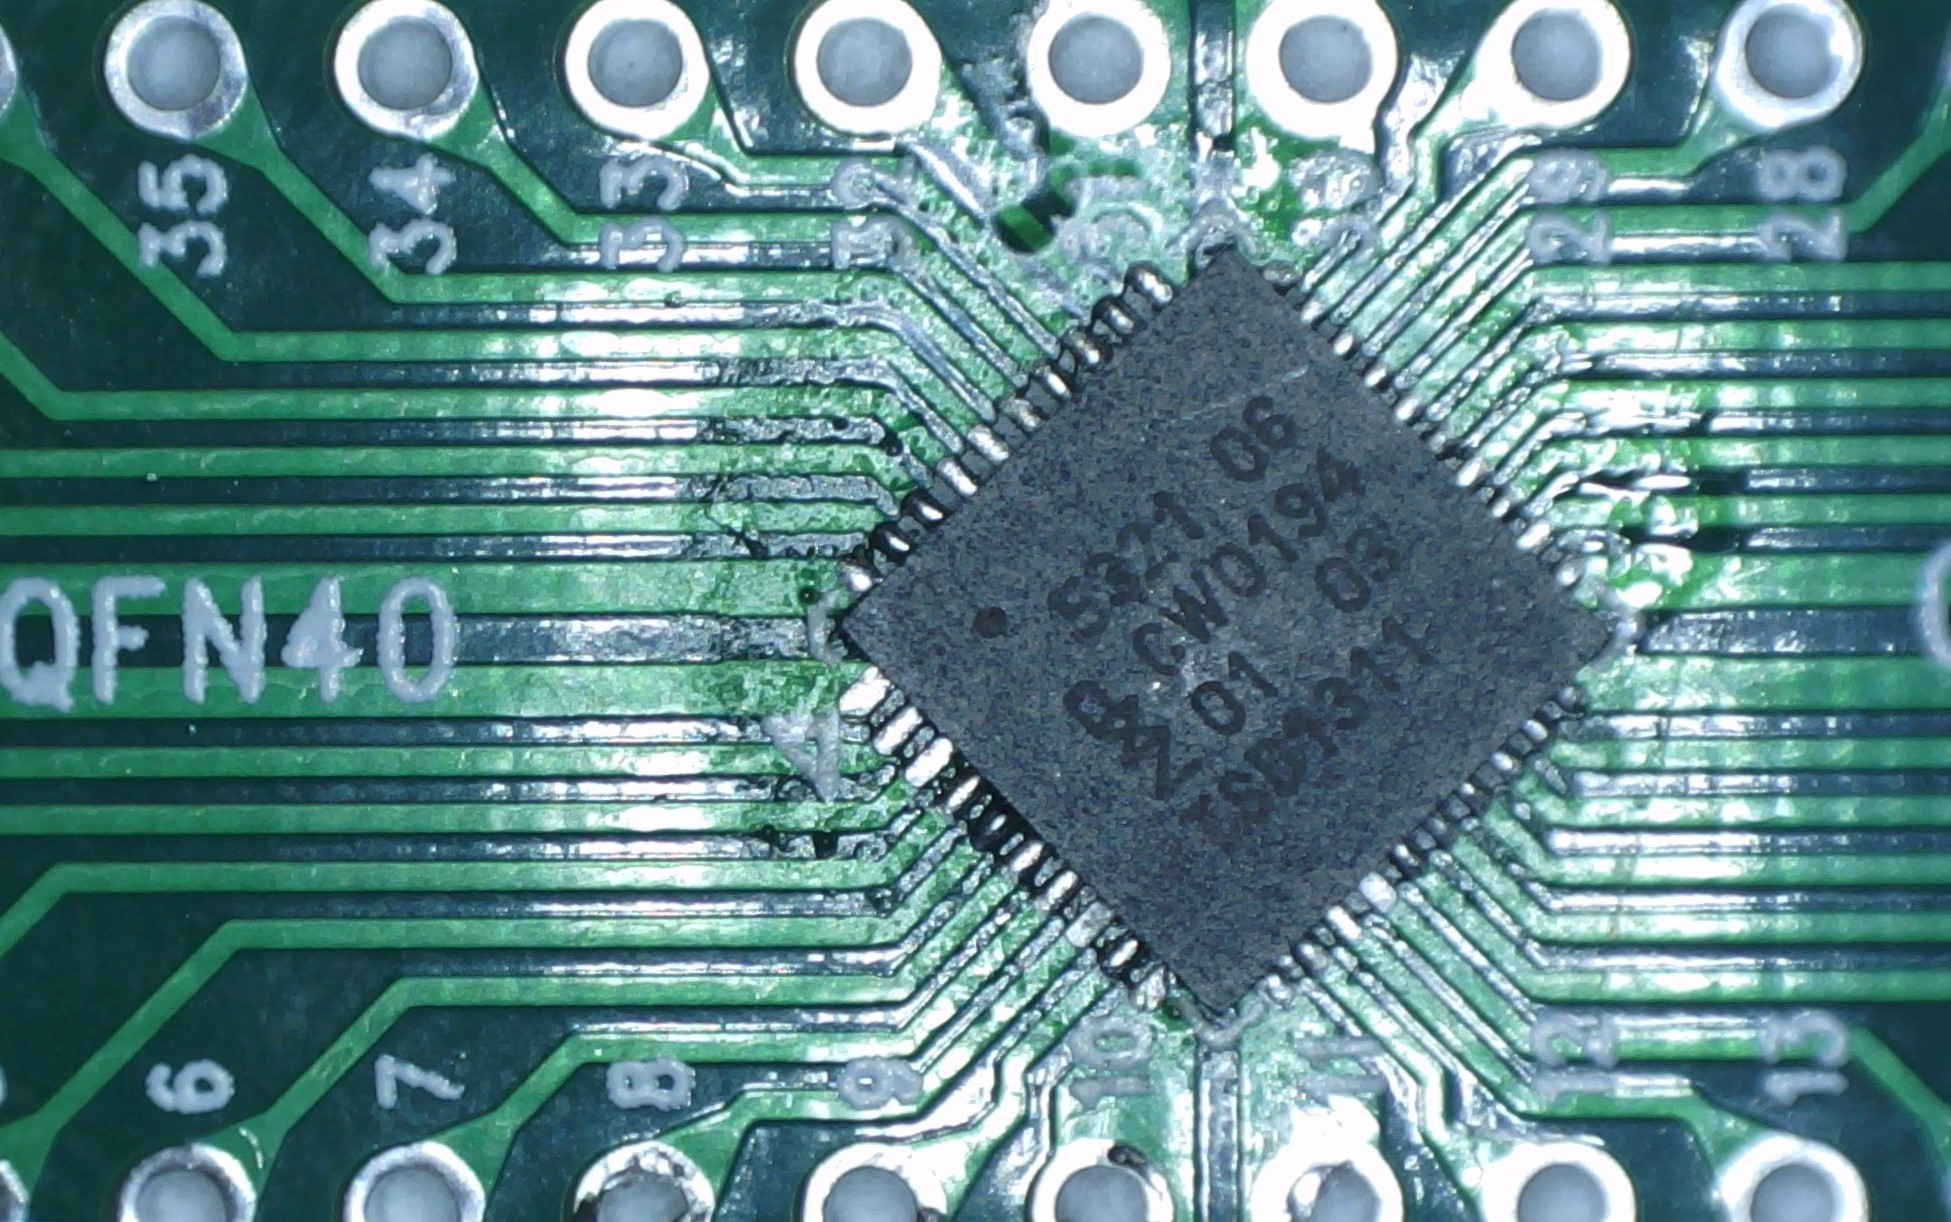
\includegraphics[scale = 0.15]{PN532}
		}
		\end{center}
		\caption{PN532}
	\end{figure}

    Since the processor translate messages of two protocol, one is from PN532 data sheet and the other is the protocol we design. Besides of strong processing ability, it also need some GPIO to control the coil selection and power on-off. For better performance and fewest foots, we use decoder such as 74HC138 to minimize foot use and use latch to control power. We have STC15W4K48S, QFP44 package, up to 33MHz 1T 8051 micro-controller.

\subsection{This is subsection}

    We have several advantages in providing a platform for IoT devices to work elegantly and efficiently, and probably to unify on-table devices with its manipulating mode, in a rather low cost and low complexity.

	\subsubsection{this is subsubsection}


p
{\small
	\bibliographystyle{ieee}
	\bibliography{SGbib}
}

\end{document}
